\documentclass{article}
%
\usepackage[mathcal,mathbf]{euler}
\usepackage{theorem,amsmath,enumerate,fancyhdr,amssymb,amsfonts}
\usepackage[pdftex]{graphics}
\usepackage{graphicx}
\usepackage{listings}
\usepackage{courier}

\usepackage{myDefs}


\lstdefinelanguage{AMPL}{keywords={set,param,var,arc,integer,minimize,maximize,subject,to,node,sum,in,Current,complements,integer,solve_result_num,IN,contains,less,suffix,INOUT,default,logical,sum,Infinity,dimen,max,symbolic
,Initial,div,min,table,LOCAL,else,option,then,OUT,environ,setof ,union,all,exists,shell_exitcodeuntil,binary,forall,solve_exitcodewhile ,by,if,solve_messagewithin,check,in,solve_result
},sensitive=true,comment=[l]{\#}}

\lstset{frame=tb,
  language=AMPL,
  aboveskip=3mm,
  belowskip=3mm,
  showstringspaces=false,
  columns=flexible,
  basicstyle={\ttfamily},
  numbers=none,
  numberstyle=\tiny\color{gray},
  keywordstyle=\bfseries,
  commentstyle=\textit,
  stringstyle=\color{mauve},
  breaklines=true,
  breakatwhitespace=true,
  tabsize=3
}


\begin{document}

\pagestyle{fancy}
\lhead{{\bf Assignment 1}
\\{\bf Author: }{Yuan Qu} } 
\rhead{{\bf Date: }01/31/2017} 

\section*{Problem 1}{
    \subsection*{a.}{
        This defines an independence system \((\mathit{E},\mathcal{F}), \mathcal{F} \subseteq \mathrm{2}^{\mathit{E}}\)\\

        First, prove that \(\emptyset \in \mathcal{F}\).

        Obviously, we have \(\emptyset \subseteq \mathit{E}=\{\mathrm{1,2,...,n}\}\), and \(\mathit{a}(\emptyset)=\sum_{\mathit{j} \in \emptyset}=\mathrm{0} \leqslant \mathit{b} \in \mathbb{R}_{+}\)

        So, \(\emptyset \in \mathcal{F}\).\\

        Second, prove that \(\mathit{X} \subseteq \mathit{Y} \in \mathcal{F} \Rightarrow \mathit{X} \in \mathcal{F}\)

        \[\mathit{Y} \in \mathcal{F} \Rightarrow \mathit{a}(\mathit{Y}) = \sum_{\mathit{j} \in \mathit{Y}}\mathit{a_j} \leqslant \mathit{b}\]

        \[\mathit{X} \subseteq \mathit{Y} \Rightarrow \mathit{a}(\mathit{X}) = \sum_{\mathit{j} \in \mathit{X}}\mathit{a_j} = \sum_{\mathit{i} \in \mathit{Y}}\mathit{a_i} - \sum_{\mathit{j} \in \mathit{Y} \setminus \mathit{X}}\mathit{a_j} \leqslant \sum_{\mathit{j} \in \mathit{Y}}\mathit{a_j} \leqslant \mathit{b}\]\\

        So, this difines an independence system \((\mathit{E},\mathcal{F}), \mathcal{F} \subseteq \mathrm{2}^{\mathit{E}}\)
    }
    \subsection*{b.}{
        According to the defination, we have
        \[\mathrm{n=6} \Rightarrow \mathit{S} \subseteq \mathit{E} = \{ \mathrm{1,2,3,4,5,6}\}\]
        \[\mathit{a}=\mathrm{(1,1,1,4,4,5), b=8} \Rightarrow \mathit{a}(\mathit{S}) = \sum_{\mathit{j} \in \mathit{S}}\mathit{a_j} \leqslant \mathrm{8}\]
        According to the defination of \textit{rank}, we have
        \[\mathit{r(X)}=\underset{\mathit{F} \in \mathcal{F}}{\mathit{max}} \lvert \mathit{F} \cap \mathit{X} \rvert=\underset{\mathit{B} \in \mathcal{B}_{\mathit{X}}} {\mathit{max}} \lvert \mathit{B} \rvert \text{, and } \mathit{\rho(X)} = \underset{\mathit{B} \in \mathcal{B}_{\mathit{X}}} {\mathit{min}} \lvert \mathit{B} \rvert\]
        We can find that
        \[\mathcal{B}_{\mathit{X}} = \mathrm{\big{\{} \{1,2,3,4\}, \{1,2,3,5\}, \{1,2,3,6\}, \{4,5\}\big{\}}}\]
        So that we have \(\mathit{r(X)}=\mathrm{4}, \mathit{\rho(X)}=\mathrm{2}\)
    }
    \subsection*{c.}{
        \[\mathit{O\big{(}r(X)\big{)}=O(n log n)}\]
        As the greedy algorithm, order the \(\mathit{a}\) from small to large, use the \textit{Best-in Greedy} to select numbers from the smallest. So the complexity is \(\mathit{O(n log n)}\)
    }
    \subsection*{d.}{
        \[\mathit{O\big{(}\rho(X)\big{)}=O(n^{\mathrm{2}})}\]
        Need to find all the subset of \(\mathit{S}\) So the complexity is \(\mathit{O(n^2)}\)
    }
    \subsection*{e.}{
        As \textit{b.} mentioned, \(\mathit{B}_{\mathrm{3}}=\mathrm{\{1,2,3,6\}},\mathit{B}_{\mathrm{4}}=\mathrm{\{4,5\}}\). If we use \textit{Best-in Greedy}, we may lose the \(\mathit{B}_{\mathrm{4}}\), because there is a solution when the first choice is 6. 
    }
}

\section*{Problem 2}{
    \subsection*{a.}{
        We have the job set \(\mathit{E}\) like following
        \begin{center}{
            \begin{tabular}{|c|c|c|c|c|c|c|c|}
            \hline
            Job & 1 & 2 & 3 & 4 & 5 & 6 & 7 \\
            \hline
            Due & 3 & 2 & 4 & 1 & 4 & 4 & 6 \\
            \hline
            Profit & 2 & 3 & 4 & 3 & 3 & 6 & 7 \\
            \hline
            \end{tabular}
        }
        \end{center} 
        The purpose is to find a independent subset \(\mathit{S} \subseteq \mathit{E}\)\\
        The initialization of \textit{Best-in Greedy} is sorting the jobs, as following
        \begin{center}{
            \begin{tabular}{|c|c|c|c|c|c|c|c|}
            \hline
            Job & 7 & 6 & 3 & 5 & 4 & 2 & 1 \\
            \hline
            Due & 6 & 4 & 4 & 4 & 1 & 2 & 3 \\
            \hline
            Profit & 7 & 6 & 4 & 3 & 3 & 3 & 2 \\
            \hline
            \end{tabular}
        }
        \end{center} 
        Then, as \textit{Best-in Greedy}, the process would be
        \begin{center}{
            \begin{tabular}{|c|c|c|c|c|}
            \hline
            Date & 1 & 2 & 3 & 4 \\
            \hline
            Job & 7 & 6 & 3 & 5 \\
            \hline
            Due & 6 & 4 & 4 & 4 \\
            \hline
            Profit & 7 & 6 & 4 & 3 \\
            \hline
            \end{tabular}
        }
        \end{center}
        The total profit would be: \(\mathrm{7+6+4+3=20}\)
    }
    \subsection*{b.}{
        Suppose \(\mathit{A}\) and \(\mathit{B}\) are two independent subsets of \(\mathit{E}\), so we have \(\mathit{A}, \mathit{B} \subseteq \mathit{E}\), and \(\mathit{A}, \mathit{B} \in \mathcal{F}\). Construct \(\mathit{A}\) and \(\mathit{B}\) as:

        \[\mathit{A}=\{ \mathit{a}_{\mathrm{1}}, \mathit{a}_{\mathrm{2}}, ..., \mathit{a}_{\mathrm{k}}\}, \mathit{B}=\{ \mathit{b}_{\mathrm{1}}, \mathit{b}_{\mathrm{2}}, ..., \mathit{b}_{\mathrm{m}}\}, \mathit{a}_{\mathrm{i}} \text{ and } \mathit{b}_{\mathrm{j}} \text{ means the job in }\mathit{A}, \mathit{B}\]

        Suppose that \(\mathrm{k} < \mathrm{m}\), so \(\lvert \mathit{A} \rvert < \lvert \mathit{B} \rvert\).

        If all the due of \(\mathit{a}_{\mathrm{i}}\) is less or equal than \(\mathrm{k}\), it's easy to find a \(\mathit{b}_{\mathrm{j}}\) whose due is larger than \(\mathrm{k}\), because of \(\mathrm{k} < \mathrm{m}\). So, we can add \(\mathit{b}_{\mathrm{j}}\) to \(\mathit{A}\) as \(\mathit{a}_{\mathrm{k+1}}\) and all the jobs can be processed, 
        \[\mathit{b}_{\mathrm{j}} \in \mathit{B} \setminus \mathit{A}, \mathit{A} \cup \{ \mathit{b}_{\mathrm{j}} \} \in \mathcal{F}\]

        If \(\exists \mathit{a}_{\mathrm{i}}, \mathit{d}_{\mathit{a}_{\mathrm{i}}}>k\), we can find a \(\mathit{b}_{\mathrm{j}} \in \mathit{B} \setminus \mathit{A}\) whose due is larger than \(\mathrm{i}\), because of \(\mathrm{k-i} < \mathrm{m-i}\). So, we can put \(\mathit{a}_{\mathrm{i}}\) as \((\mathrm{k+1})\)th process and set \(\mathit{b}_{\mathrm{j}}\) as \(\mathrm{i}\)th process, all the jobs can be processed,
        \[\mathit{b}_{\mathrm{j}} \in \mathit{B} \setminus \mathit{A}, \mathit{A} \cup \{ \mathit{b}_{\mathrm{j}} \} \in \mathcal{F}\]

        So, \((\mathit{E},\mathcal{F})\) is a matroid.
    }
}

\section*{Problem 3}{
    \subsection*{a.}{
        \(\big{(}\mathit{V(G)},\mathcal{F}\big{)}\) is a matroid.\\

        First, prove that \(\emptyset \in \mathcal{F}\).

        Obviously, we have \(\emptyset \subseteq \mathit{V(G)}\), and there is no edge because of no vertex. 

        So, \(\emptyset \in \mathcal{F}\).\\

        Second, prove that \(\mathit{X} \subseteq \mathit{Y} \in \mathcal{F} \Rightarrow \mathit{X} \in \mathcal{F}\)

        If \(\mathit{Y}\) is independent, which means no edge inside the \(\mathit{Y}\), obviously all the subsets of \(\mathit{Y}\) contain no edge inside.

        So, this difines an independence system \(\big{(}\mathit{V(G)},\mathcal{F}\big{)}, \mathcal{F} \subseteq \mathrm{2}^{\mathit{V(G)}}\)\\

        Third, to prove that the independence system \(\big{(}\mathit{V(G)},\mathcal{F}\big{)}\) is a matroid, according to the \textit{lemma 2}, only need to prove \textbf{for each \(\mathit{X} \subseteq \mathit{E}\), all bases of \(\mathit{X}\) are of the same size.}

        Supposed \(\lvert \mathit{V(G)} \rvert = \mathrm{n}\). 

        Apparently, no matter which vertices are chosen, for \(\mathrm{n}\) is \textit{odd}, the size of all the bases of \(\mathit{X}\) is equal to \(\frac{\mathit{n}-\mathrm{1}}{\mathrm{2}}\), and for \(\mathrm{n}\) is \textit{even}, the size of all the bases of \(\mathit{X}\) is equal to \(\frac{\mathit{n}}{\mathrm{2}}\).\\

        So, \(\big{(}\mathit{V(G)},\mathcal{F}\big{)}\) is a matroid.
    }
    \subsection*{b.}{
        While \(\mathit{n} = \mathrm{5}\), according to \textit{a.}, so that the size of bases \(\mathit{r(S)} = \frac{\mathit{n}-\mathrm{1}}{\mathrm{2}}=\mathrm{2}\).

        Therefore, the defining inequalities for \(\mathit{P}_{\mathit{V(G)},\mathcal{F}}\):

        \[\mathit{S}_{\mathrm{1}} = \{ \mathit{x}_{\mathrm{1}}, \mathit{x}_{\mathrm{3}}\} \quad \mathit{x}(\mathit{S}_{\mathrm{1}}) = \mathit{x}_{\mathrm{1}} + \mathit{x}_{\mathrm{3}} \leqslant \mathit{r(S)} = 2\]

        \[\mathit{S}_{\mathrm{2}} = \{ \mathit{x}_{\mathrm{2}}, \mathit{x}_{\mathrm{4}}\} \quad \mathit{x}(\mathit{S}_{\mathrm{2}}) = \mathit{x}_{\mathrm{2}} + \mathit{x}_{\mathrm{4}} \leqslant \mathit{r(S)} = 2\]

        \[\mathit{S}_{\mathrm{3}} = \{ \mathit{x}_{\mathrm{3}}, \mathit{x}_{\mathrm{5}}\} \quad \mathit{x}(\mathit{S}_{\mathrm{3}}) = \mathit{x}_{\mathrm{3}} + \mathit{x}_{\mathrm{5}} \leqslant \mathit{r(S)} = 2\]

        \[\mathit{S}_{\mathrm{4}} = \{ \mathit{x}_{\mathrm{4}}, \mathit{x}_{\mathrm{1}}\} \quad \mathit{x}(\mathit{S}_{\mathrm{4}}) = \mathit{x}_{\mathrm{4}} + \mathit{x}_{\mathrm{1}} \leqslant \mathit{r(S)} = 2\]

        \[\mathit{S}_{\mathrm{5}} = \{ \mathit{x}_{\mathrm{5}}, \mathit{x}_{\mathrm{2}}\} \quad \mathit{x}(\mathit{S}_{\mathrm{5}}) = \mathit{x}_{\mathrm{5}} + \mathit{x}_{\mathrm{2}} \leqslant \mathit{r(S)} = 2\]
    }
    \subsection*{c.}{
        Yes. According to the \textit{Edmonds(1970)} The output is the linear, especially binary in this case, combination of the characteristic vectors, which are integral. So the ploytope \(\mathit{P}_{\mathit{V(G)},\mathcal{F}}\) is integral.
    }
}

\section*{Problem 4}{
    As the defination, the graph is following.
    \begin{center}{
        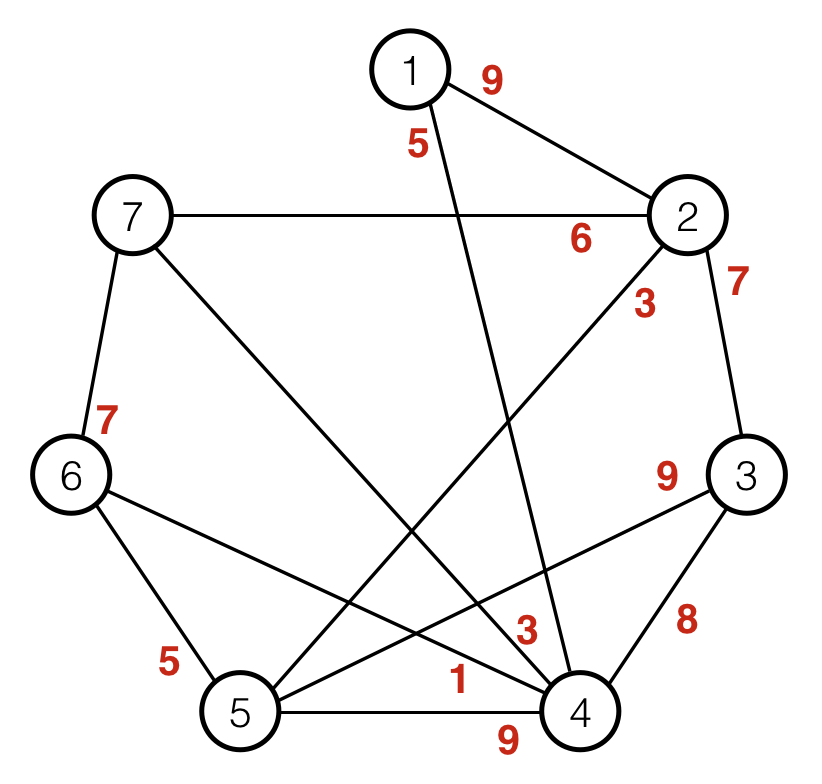
\includegraphics[scale=0.5]{P4.png}
    }
    \end{center}
    Use \textit{Kruskal's Algorithm} to find the maximum-weight spanning tree.

    \paragraph{Initialize}{
        Sort \(\mathit{E}\) by weight from largest to smallest. 
        \[\mathit{E} = \big{\{} (1,2), (3,5), (4,5), (3,4), (2,3), (6,7), (2,7), (1,4), (5,6), (2,5), (4,7), (4,6)\big{\}}\]
        Set \(\mathit{T}=\emptyset\)

        \begin{enumerate}{
            \item \(\mathit{T} \cup \{ (1,2) \} \), cycle free, \(\mathit{T} = \mathit{T} \cup \{ (1,2) \} \)
            \item \(\mathit{T} \cup \{ (3,5) \} \), cycle free, \(\mathit{T} = \mathit{T} \cup \{ (3,5) \} \)
            \item \(\mathit{T} \cup \{ (4,5) \} \), cycle free, \(\mathit{T} = \mathit{T} \cup \{ (4,5) \} \)
            \item \(\mathit{T} \cup \{ (3,4) \} \), cycle!
            \item \(\mathit{T} \cup \{ (2,3) \} \), cycle free, \(\mathit{T} = \mathit{T} \cup \{ (2,3) \} \)
            \item \(\mathit{T} \cup \{ (6,7) \} \), cycle free, \(\mathit{T} = \mathit{T} \cup \{ (6,7) \} \)
            \item \(\mathit{T} \cup \{ (2,7) \} \), cycle free, \(\mathit{T} = \mathit{T} \cup \{ (2,7) \} \)
            \item \(\mathit{T} \cup \{ (1,4) \} \), cycle! No alone vertex, means rest edges make cycle, algorithm end.
        }
        \end{enumerate}
        So that the \(\mathit{T} = \{ (1,2), (3,5), (4,5), (2,3), (6,7), (2,7)\} \)

        The weight of the maximum-weight spanning tree is
        \[\mathit{w}_{1,2}+\mathit{w}_{3,5}+\mathit{w}_{4,5}+\mathit{w}_{2,3}+\mathit{w}_{6,7}+\mathit{w}_{2,7} = 47\]
    }
}

\section*{Problem 5}{
    \subsection*{a.}{
        \[\lvert \mathit{B} \rvert = \mathrm{\frac{15 \times 3 + 18 \times 5 + 12 \times 15}{1+2+4} = 45}\]
    }
    \subsection*{b.}{
        The maximum cardinality matching in this graph is 45. \\

        If graph \( \mathit{G} = (\mathit{A} \cup \mathit{B}, \mathit{E})\) has a \textit{Perfect Matching}, which has \(\nu (\mathit{G}) = \lvert \mathit{A} \rvert\), the maximum cardinality matching will be \textit{Perfect Matching}. 

        Now prove that in this case \( \mathit{G} = (\mathit{A} \cup \mathit{B}, \mathit{E})\) has a \textit{Perfect Matching}.

        According to \textit{Theorem 3 (Frobeiniu(1971), Hall(1935))}, only need to prove, 
        \[\lvert \mathit{S} \rvert \leqslant \lvert \mathit{N(S)} \rvert \quad \text{for all} \quad \mathit{S} \subseteq \mathit{A}\]

        Proof by contradiction. If \(\exists \lvert \mathit{S} \rvert > \lvert \mathit{N(S)} \rvert, \mathit{S} \subseteq \mathit{A}\). Suppose that \(\mathrm{k} = \lvert \mathit{S} \rvert, \mathrm{m} = \lvert \mathit{N(S)} \rvert\), i.e. \(\mathrm{k} > \mathrm{m}\). 

        Suppose that \[\mathit{k}_{\mathrm{1}} + \mathit{k}_{\mathrm{2}} + \mathit{k}_{\mathrm{3}} = \mathit{k} > \mathit{m}\]

        in which \(\mathit{k}_{\mathrm{1}}\) refers the number of vertices of degree 3, \(\mathit{k}_{\mathrm{2}}\) refers the number of vertices of degree 5, \(\mathit{k}_{\mathrm{3}}\) refers the number of vertices of degree 15.

        According to the defination of \(\mathit{B}\), we could get \(\mathit{m} \geqslant \mathrm{3}\mathit{k}_{\mathrm{1}}\), \(\mathit{m} \geqslant \mathrm{\frac{5}{2}}\mathit{k}_{\mathrm{2}}\), \(\mathit{m} \geqslant \mathrm{\frac{15}{4}}\mathit{k}_{\mathrm{3}}\), so we have 

        \[\mathit{m} = \mathrm{(\frac{1}{3} + \frac{2}{5} + \frac{4}{15})}\mathit{m} \geqslant \mathit{k}_{\mathrm{1}} + \mathit{k}_{\mathrm{2}} + \mathit{k}_{\mathrm{3}} = \mathit{k} > \mathit{m}\]

        Which makes \(\mathit{m} > \mathit{m}\), \textbf{contradiction}.

        So graph \( \mathit{G} = (\mathit{A} \cup \mathit{B}, \mathit{E})\) has a \textit{Perfect Matching}, and \(\nu (\mathit{G}) = \lvert \mathit{A} \rvert\).
    }
}

\section*{Problem 6}{
    Use AMPL model to solve this problem. \\

    Code :

    \begin{lstlisting}[language=AMPL]
#File: CuttingStock.mod
#Date: 2017.03.16
#Author: Yuan Qu

#-----CUTTING STOCK MODEL USING PATTERNS-----
param roll_width >0;

set WIDTHS;
param orders {WIDTHS} >0;

param nPAT integer >=0;
set PATTERNS := 1..nPAT;

param A{WIDTHS, PATTERNS} integer >=0;
    check{j in PATTERNS}:
        sum {i in WIDTHS} i * A[i,j] <= roll_width;
        
var X{PATTERNS} integer >=0;

minimize NumberOfRolls:
    sum {j in PATTERNS} X[j];

subj to OrderFill {i in WIDTHS}:
    sum {j in PATTERNS} A[i,j] * X [j] >=orders[i];

#-----KNAPSACK SUBPROLEM FOR CUTTING STOCK-----
param dualprice {WIDTHS} default 0.0;

var C {WIDTHS} integer >=0;

minimize Reduced_Cost:
    1 - sum {i in WIDTHS} dualprice[i] * C[i];

subj to Width_Limit:
    sum {i in WIDTHS} i * C[i]  <=roll_width;

#-----Reading Data and Choosing Solver---------
data CuttingStock.dat;

option solver cplex;
option solution_round 6;

#-----Defining the Two Stages------------------
problem Cutting_Opt: X, NumberOfRolls, OrderFill;
option relax_integrality 1;

problem Pattern_Gen: C, Reduced_Cost, Width_Limit;
option relax_integrality 0;

#-----Initializing Pattern Set-----------------
let nPAT := 0;

for {i in WIDTHS} {
   let nPAT := nPAT + 1;
   let A[i,nPAT] := floor (roll_width/i);
   let {i2 in WIDTHS: i2 <> i} A[i2,nPAT] := 0;
};

#-----Two Stage Optimization Loop--------------
repeat {
   solve Cutting_Opt;

   let {i in WIDTHS} dualprice[i] := OrderFill[i].dual;

   solve Pattern_Gen;

   if Reduced_Cost < -0.00001 then {
      let nPAT := nPAT + 1;
      let {i in WIDTHS} A[i,nPAT] := C[i];
      
      display C;
   }
   else break;
};

#-----Final Integer Program with Generated Patterns------
option Cutting_Opt.relax_integrality 0;
solve Cutting_Opt;

#-----Displaying Results---------------------------------
display A; 
display X;
    \end{lstlisting}

    Data:
    \begin{lstlisting}[language=AMPL]
#File: CuttingStock.dat
#Date: 2017.03.16
#Author: Yuan Qu

param roll_width := 24 ;

param: WIDTHS: orders :=
          3     12300
          5     9800
          12    3600
          7     5750
          8     15250
          9     6700 ;

    \end{lstlisting}

    Result:

    In this part, \(\mathit{A}\) means the Patterns, in which \(\mathit{A[i,j]}\) refers in Pattern \(\mathit{i}\), the cut number of Width \(\mathit{j}\). \(\mathit{X}\) means the optimal solution, in which \(\mathit{X[i]}\) refers the number of Pattern \(\mathit{i}\) processed.

    The processing result during the iteration is not copied.
    \begin{lstlisting}
A [*,*] (tr)
:    3   5   7   8   9  12    :=
1    8   0   0   0   0   0
2    0   4   0   0   0   0
3    0   0   0   0   0   2
4    0   0   3   0   0   0
5    0   0   0   3   0   0
6    0   0   0   0   2   0
7    0   1   0   0   2   0
8    0   2   2   0   0   0
9    1   4   0   0   0   0
10   0   3   0   0   1   0
11   2   0   0   0   2   0
;

X [*] :=
 1   869
 2     0
 3  1800
 4     0
 5  5084
 6     0
 7     0
 8  2875
 9     0
10  1350
11  2675
;
    \end{lstlisting}
}

\section*{Problem 7}{
    Use AMPL model to solve this problem. \\

    Code :
    \begin{lstlisting}[language=AMPL]
#File: P7.mod
#Date: 2017.03.16
#Author: Yuan Qu

param total >0;
set ID;

param profit {ID} > 0;
param cost {ID} > 0;
param f_min {ID} >= 0;
param f_max {j in ID} >= f_min[j];

var Invest {j in ID} integer >= f_min[j], <= f_max[j];

maximize Total_Profit: sum {j in ID} profit[j] * Invest[j];

subject to Total_Cost: sum {j in ID} cost[j] * Invest[j] <= total ;

data P7.dat;

option solver cplex;
solve;

display Total_Profit;
display Invest;
    \end{lstlisting}

    Data:
    \begin{lstlisting}[language=AMPL]
#File: P7.dat
#Date: 2017.03.16
#Author: Yuan Qu

param total := 100 ;

set ID := A B C D E F G H I J K L;
param: profit   cost    f_min   f_max :=
    A   30      16      0       1
    B   25      15      0       1
    C   5       2       0       1
    D   9       4       0       1
    E   11      4       0       1
    F   7       3       0       1
    G   14      9       0       1
    H   19      12      0       1
    I   40      29      0       1
    J   29      20      0       1
    K   30      18      0       1
    L   34      25      0       1;
    \end{lstlisting}

    Result: it means the max total profit is 172 by investing \(\{ \mathit{A}, \mathit{B}, \mathit{C}, \mathit{D}, \mathit{E}, \mathit{G}, \mathit{H}, \mathit{J}, \mathit{K}\}\)
    \begin{lstlisting}[language=AMPL]
CPLEX 12.7.0.0: optimal integer solution; objective 172
5 MIP simplex iterations
0 branch-and-bound nodes
No basis.
Total_Profit = 172

Invest [*] :=
A  1
B  1
C  1
D  1
E  1
F  0
G  1
H  1
I  0
J  1
K  1
L  0
;
\end{lstlisting}
}

\section*{Problem 8}{
    Use AMPL model to solve this problem. \\

    Code:

    In this part, couldn't find a concise way to organize the model, so the code is simple and redundant.

    By the way, find that the result will be same if there is no multiple limitation of \textit{own power plants} and \textit{rent power plants}, so there is no limitation in code.
    \begin{lstlisting}[language=AMPL]
#File: P8.mod
#Date: 2017.03.17
#Author: Yuan Qu

#The demand for 1-7 days
param d1 = 1230; 
param d2 = 1190;
param d3 = 845;
param d4 = 935;
param d5 = 915;
param d6 = 1625;
param d7 = 1510;

#The own plants for 1-7 days
var o1 integer >= 0, <= 500;
var o2 integer >= 0, <= 500;
var o3 integer >= 0, <= 500;
var o4 integer >= 0, <= 500;
var o5 integer >= 0, <= 500;
var o6 integer >= 0, <= 500;
var o7 integer >= 0, <= 500;

#The rent plants for 1-7 days
var r1 integer >= 0, <= 600;
var r2 integer >= 0, <= 600;
var r3 integer >= 0, <= 600;
var r4 integer >= 0, <= 600;
var r5 integer >= 0, <= 600;
var r6 integer >= 0, <= 600;
var r7 integer >= 0, <= 600;

#The purchase(buy) plants for 1-7 days
var b1 integer >= 0, <= 500;
var b2 integer >= 0, <= 500;
var b3 integer >= 0, <= 500;
var b4 integer >= 0, <= 500;
var b5 integer >= 0, <= 500;
var b6 integer >= 0, <= 500;
var b7 integer >= 0, <= 500;

#Store of electricity for 1-7 days, cumulative
var s1 integer >= 0;
var s2 integer >= 0;
var s3 integer >= 0;
var s4 integer >= 0;
var s5 integer >= 0;
var s6 integer >= 0;
var s7 integer >= 0;

#Objective Function
minimize Cost: 20*(o1+o2+o3+o4+o5+o6+o7) + 25*(r1+r2+r3+r4+r5+r6+r7) + 45*(b1+b2+b3+b4+b5+b6+b7) + 2*(s1+s2+s3+s4+s5+s6+s7);

#Constraints of the defination of store
subject to Store1: s1 = o1 + r1 + b1 - d1;
subject to Store2: s2 = o2 + r2 + b2 + s1 - d2;
subject to Store3: s3 = o3 + r3 + b3 + s2 - d3;
subject to Store4: s4 = o4 + r4 + b4 + s3 - d4;
subject to Store5: s5 = o5 + r5 + b5 + s4 - d5;
subject to Store6: s6 = o6 + r6 + b6 + s5 - d6;
subject to Store7: s7 = o7 + r7 + b7 + s6 - d7;

#Constraints that fill the demand
subject to Demand1: o1 + r1 + b1 >= d1;
subject to Demand2: o2 + r2 + b2 + s1 >= d2;
subject to Demand3: o3 + r3 + b3 + s2 >= d3;
subject to Demand4: o4 + r4 + b4 + s3 >= d4;
subject to Demand5: o5 + r5 + b5 + s4 >= d5;
subject to Demand6: o6 + r6 + b6 + s5 >= d6;
subject to Demand7: o7 + r7 + b7 + s6 >= d7;

#Use cplex to colve integer program
option solver cplex;
solve;

display Cost;

display o1,o2,o3,o4,o5,o6,o7;
display r1,r2,r3,r4,r5,r6,r7;
display b1,b2,b3,b4,b5,b6,b7;
display s1,s2,s3,s4,s5,s6,s7;
    \end{lstlisting}

    Result:
    \begin{lstlisting}[language=AMPL]
CPLEX 12.7.0.0: optimal integer solution; objective 202470
7 MIP simplex iterations
0 branch-and-bound nodes
No basis.
Cost = 202470

o1 = 500
o2 = 500
o3 = 500
o4 = 500
o5 = 500
o6 = 500
o7 = 500

r1 = 600
r2 = 600
r3 = 600
r4 = 600
r5 = 600
r6 = 600
r7 = 600

b1 = 130
b2 = 90
b3 = 0
b4 = 0
b5 = 0
b6 = 0
b7 = 330

s1 = 0
s2 = 0
s3 = 255
s4 = 420
s5 = 605
s6 = 80
s7 = 0
    \end{lstlisting}
}

\section*{Problem 9}{

}

\section*{Problem 10}{
    \begin{center}{
        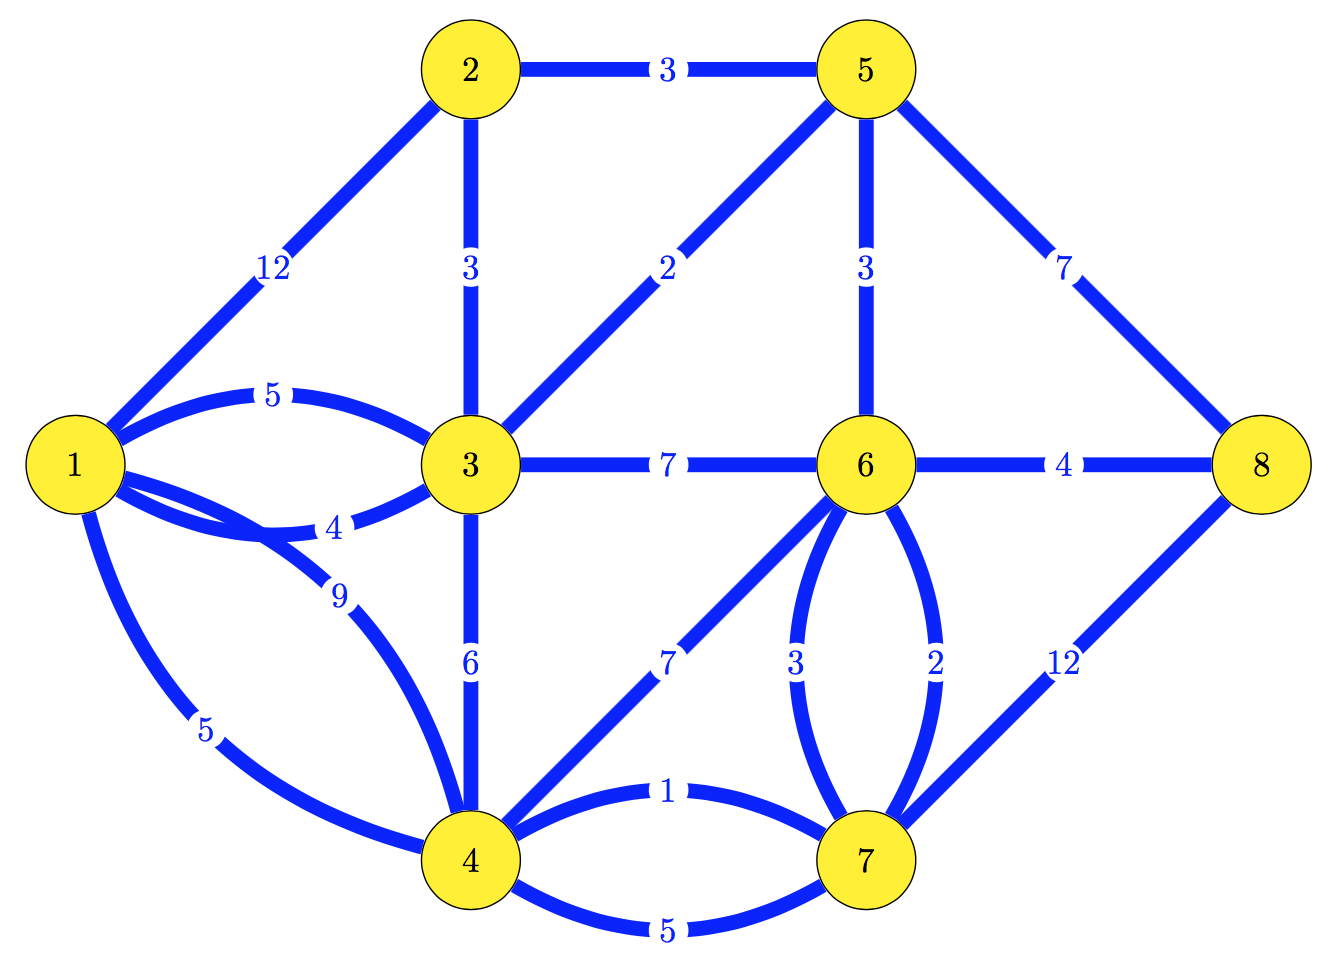
\includegraphics[scale=0.4]{P10.png}
    }
    \end{center}
    \subsection*{a.}{
        Because the vertices \(\mathit{V}_{\mathrm{1}}, \mathit{V}_{\mathrm{2}}, \mathit{V}_{\mathrm{7}}, \mathit{V}_{\mathrm{8}}\) have odd degree, so there is no \textit{Eulerian path} in this Graph \(\mathit{G}\). 

        So, to get the optimal solution of \textit{Chinese Postman Problem}, we need to consider the \(\mathit{K}_{\mathrm{4}}\), the The complete graph on \(\mathrm{4}\) vertices of \(\mathit{V}_{\mathrm{1}}, \mathit{V}_{\mathrm{2}}, \mathit{V}_{\mathrm{7}}, \mathit{V}_{\mathrm{8}}\).

        \begin{center}{
            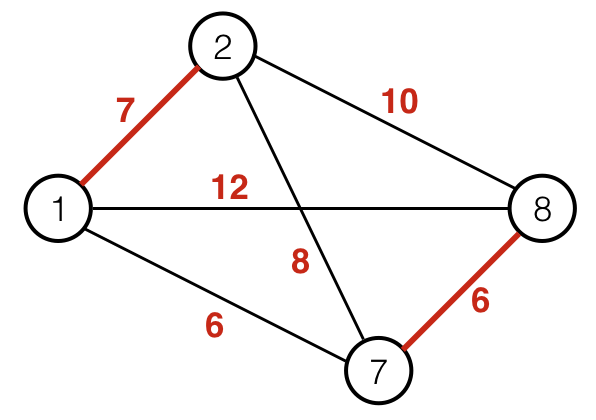
\includegraphics[scale=0.6]{P10_1.png}
        }
        \end{center}

        According to that, we choose path \(\mathit{V}_{\mathrm{1}} \to \mathit{V}_{\mathrm{2}}\) and \(\mathit{V}_{\mathrm{7}} \to \mathit{V}_{\mathrm{8}}\) to add on (means repeat) the orginal graph.

        \begin{center}{
            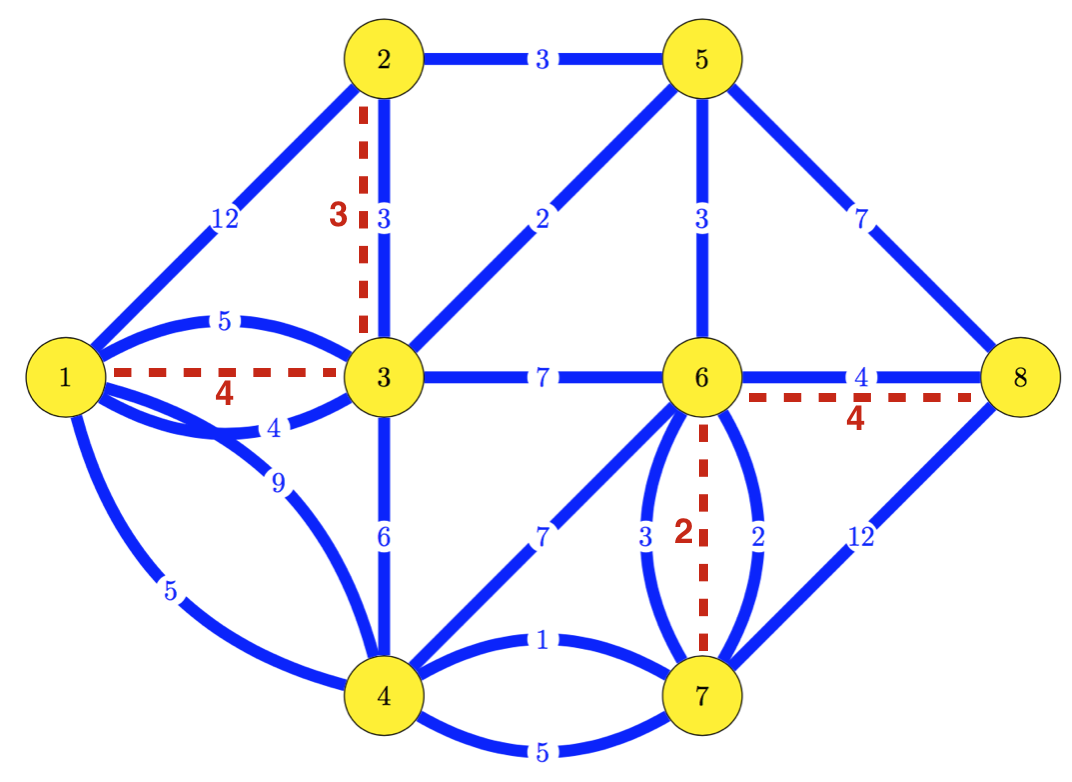
\includegraphics[scale=0.6]{P10_2.png}
        }
        \end{center}

        In this case, it's easy to find a \textit{Eulerian path} that:
        \[\mathit{V}_{\mathrm{1}} \to \mathit{V}_{\mathrm{2}} \to \mathit{V}_{\mathrm{5}} \to \mathit{V}_{\mathrm{8}} \to \mathit{V}_{\mathrm{6}} \to \mathit{V}_{\mathrm{5}} \to \mathit{V}_{\mathrm{3}} \to \mathit{V}_{\mathrm{6}} \to \mathit{V}_{\mathrm{8}} \to \mathit{V}_{\mathrm{7}} \to \mathit{V}_{\mathrm{6}} \to \mathit{V}_{\mathrm{7}}\]
        \[\to \mathit{V}_{\mathrm{6}} \to \mathit{V}_{\mathrm{4}} \to \mathit{V}_{\mathrm{7}} \to \mathit{V}_{\mathrm{4}} \to \mathit{V}_{\mathrm{3}} \to \mathit{V}_{\mathrm{2}} \to \mathit{V}_{\mathrm{3}} \to \mathit{V}_{\mathrm{1}} \to \mathit{V}_{\mathrm{3}} \to \mathit{V}_{\mathrm{1}} \to \mathit{V}_{\mathrm{4}} \to \mathit{V}_{\mathrm{1}}\]

        Total time: 
        \[\sum_{\mathit{E}\in\mathit{G}}\mathit{w_E} + \mathit{w}_{\mathit{V}_{\mathrm{1}} \to \mathit{V}_{\mathrm{2}}} + \mathit{w}_{\mathit{V}_{\mathrm{7}} \to \mathit{V}_{\mathrm{8}}} = \mathrm{100 + 7 + 6 = 113}\]
    }
    \subsection*{b.}{
        To end in area 8, consider a \textit{Eulerian path} that the last step is \(\mathit{V}_{\mathrm{8}} \to \mathit{V}_{\mathrm{1}}\), which means \(\mathit{V}_{\mathrm{1}} \text{ and } \mathit{V}_{\mathrm{2}}\) are neighbors there is a edge between them. Because we don't need to go back area 1, so set \(\mathit{w}_{(\mathit{V}_{\mathrm{1}}, \mathit{V}_{\mathrm{8}})} = \infty \). Now \(\mathit{G}\) looks like:

        \begin{center}{
            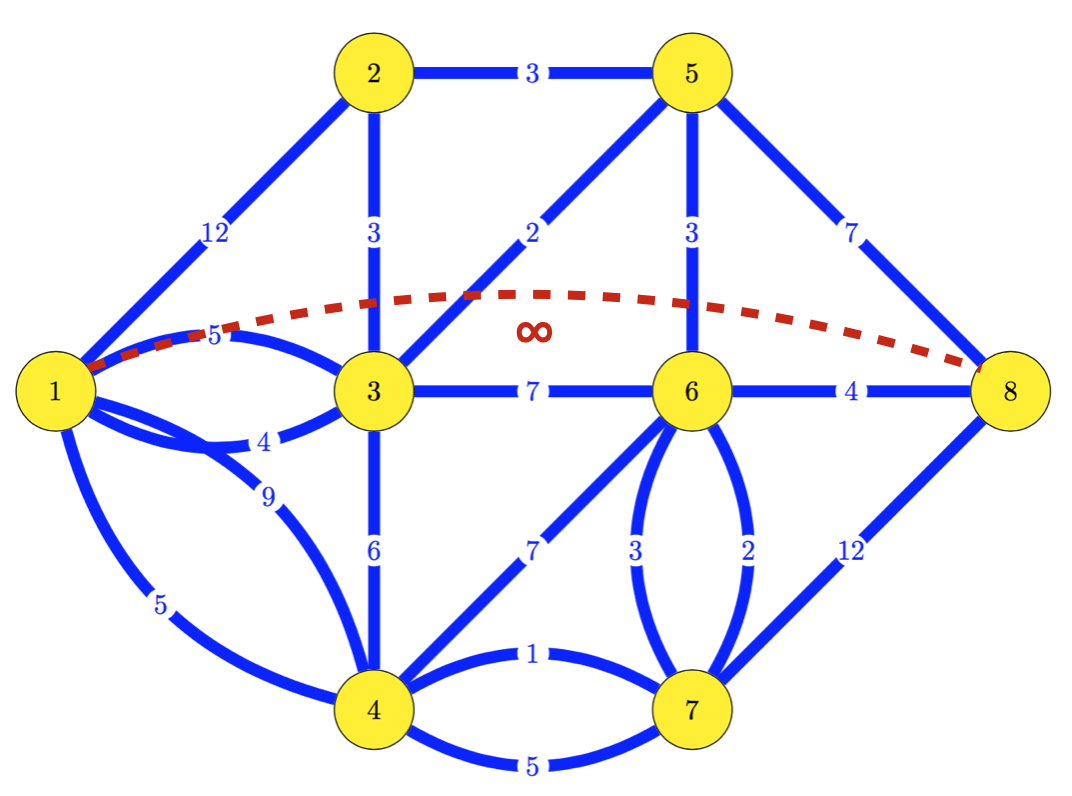
\includegraphics[scale=0.6]{P10_3.png}
        }
        \end{center}

        Construct a \textit{Eulerian path} from Graph \(\mathit{G}\), same with \textit{a.}, construct a \(\mathit{K}_{\mathrm{4}}\), the The complete graph on \(\mathrm{4}\) vertices of \(\mathit{V}_{\mathrm{1}}, \mathit{V}_{\mathrm{2}}, \mathit{V}_{\mathrm{7}}, \mathit{V}_{\mathrm{8}}\).

        \begin{center}{
            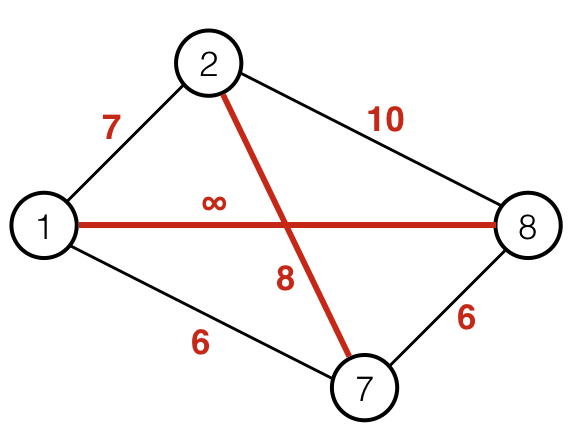
\includegraphics[scale=0.6]{P10_4.png}
        }
        \end{center}

        Because we have to choose \(\mathit{V}_{\mathrm{1}} \to \mathit{V}_{\mathrm{8}}\) as the last step, so we have to choose \(\mathit{V}_{\mathrm{2}} \to \mathit{V}_{\mathrm{7}}\) as the another route.

        So in this case, the \textit{Eulerian path} is:
        \[\mathit{V}_{\mathrm{1}} \to \mathit{V}_{\mathrm{2}} \to \mathit{V}_{\mathrm{3}} \to \mathit{V}_{\mathrm{1}} \to \mathit{V}_{\mathrm{3}} \to \mathit{V}_{\mathrm{4}} \to \mathit{V}_{\mathrm{1}} \to \mathit{V}_{\mathrm{4}} \to \mathit{V}_{\mathrm{6}} \to \mathit{V}_{\mathrm{7}} \to \mathit{V}_{\mathrm{4}} \to \mathit{V}_{\mathrm{7}}\]
        \[\to \mathit{V}_{\mathrm{6}} \to \mathit{V}_{\mathrm{3}} \to \mathit{V}_{\mathrm{5}} \to \mathit{V}_{\mathrm{2}} \to \mathit{V}_{\mathrm{5}} \to \mathit{V}_{\mathrm{6}} \to \mathit{V}_{\mathrm{5}} \to \mathit{V}_{\mathrm{8}} \to \mathit{V}_{\mathrm{6}} \to \mathit{V}_{\mathrm{7}} \to \mathit{V}_{\mathrm{8}} \to \mathit{V}_{\mathrm{1}}\]

        The optimal path is elimate the last step to \(\mathit{V}_{\mathrm{1}}\) from the \textit{Eulerian path}. And the total time is:
        \[\sum_{\mathit{E}\in\mathit{G}}\mathit{w_E} + \mathit{w}_{\mathit{V}_{\mathrm{2}} \to \mathit{V}_{\mathrm{7}}} = \mathrm{100 + 8 = 108}\]
    }

}



\end{document}
